\chapter{Defining the general use cases}
\label{ch:usecases}

\section{Supplantive or generative}

The first important design choice which has to be made is whether the students are supplied with a concept map or flashcards, or that they generate the content themselves. The dichotomy of generative versus supplantive instruction is described in further detail by \citeA{instructionaldesign}, where the implications of both sides are enlisted for the learner, the task and the context.

One of the aspects of generative strategies is that the learner requires a higher amount of prior knowledge, a higher aptitude, and a wider and more flexible range of cognitive strategies, because the content still has to be (partly) researched and constructed. This can be a disadvantage, because the learner might not possess these skills and therefore the instruction may not be suitable or highly inefficient using generative strategies. On the other hand, greater mental effort generally leads to greater depth of processing and therefore better, more meaningful learning, which was also stressed by \citeA{canas} and \citeA{nesbit}. Furthermore, learners experience a higher motivation and a lower amount of anxiety when using generative strategies, and their attribution of success is internal rather than external. 

Furthermore, when using more generative strategies, the learning task becomes more complex and ill-structured, and therefore requires more instruction and time to complete. It also leads to a higher focus on cognitive strategies, but less so on the learning goals. These goals can also not become universal, since each student creates their own flashcards or concept map, and therefore decides on their own learning content.

The most important factor for this design choice is feasibility. The teacher already stated that there is only limited time available during the lesson to introduce them to the software, so there is no time for extensive instruction on how to create concept maps, let alone creating the maps within the classroom. Additionally, students do not have much time at home to spend on creating the maps, and it is also known from both interviews with the teacher as literature that they will probably have only a low amount of intrinsic motivation. Finally, when the students have to create their own maps, it cannot be guaranted that they will include the nodes relevant for the goals of the instruction, and might become either to narrow or to extensive in certain branches. The same arguments are valid for letting students create their own flashcards. Therefore, despite of the benefits that a more generative approach may have for the learning process, the content will be supplied to the students instead.

\section{Choice of platform}

The next design decision is centered around the choice of platform or medium going to be used in order to support the learning tool. In the section \nameref{subsec:fcapplication} on page~\pageref{subsec:fcapplication} it is described that students generally prefer to use traditional or written flashcards, despite the many advantages of digital flashcards. However, with the flashmap tool this is not a feasible option, since the tool has to dynamically generate different graphs based on the general concept map and the profile of the students. Of course it would be possible to provide the concept map digitally and the flashcards in written form, however this would introduce an extra variable to the research design. Finally, with written flashcards one can only use rather crude methods for rescheduling the cards, instead of using the more precise algorithms possible within a digital tool.

There are various options for the specific implementation, for example a computer program or an app. Of these options, a web application is the most convenient, since it is accessible for any device with a modern web browser, and immediately stores the usage data on a centralised server so that it is immediately accessible for the researcher. Furthermore, adjustments or fixes can be applied during the research, without all users having to update to the newest version.

For the client, HTML, CSS, and Javascript are used, importing the vis.js library for visualising the concept map dynamically\footnote{\url{http://www.visjs.org/}}. Furthermore, Python is used for the server logic, communicating with the webclient through a websocket using JSON messages. The choice for Python is mainly based on preference by the programmer. Finally, MongoDB was used as a database engine since it stores data in a format very similar to JSON, which is also used by vis.js to represent concept maps.

The server implementation will be further elaborated in the \nameref{ch:server} chapter on page~\pageref{ch:server}, and the client implementation in the \nameref{ch:client} chapter on page~\pageref{ch:client}.

\section{Supported user actions}

The final design decision related to the general ideation of software is deciding which use cases should be supported, which are generally displayed within a UML use case diagram \cite{uml}. For the flashmap software, the use cases are divided in cases related to the registering and login process (see figure~\ref{fig:loginusecase}), and the cases related to the main use of the software (see figure~\ref{fig:mainusecase}).

\begin{figure}[h!]
\centering
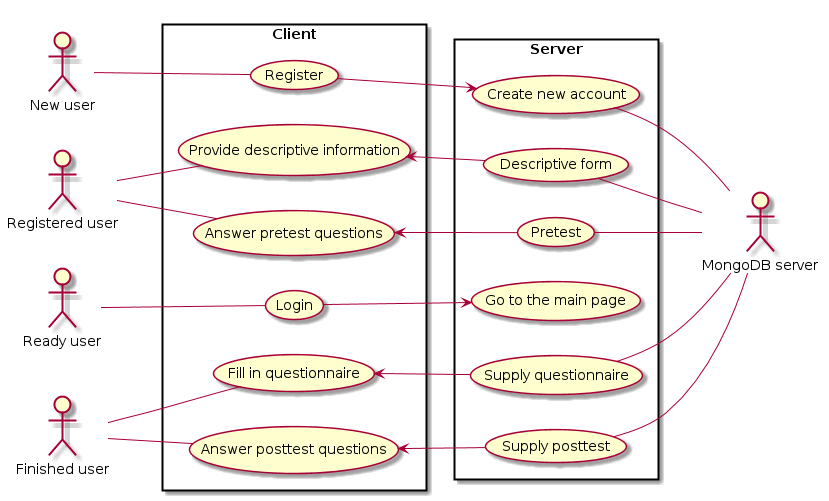
\includegraphics[width=\textwidth]{img/loginusecase.png}
\caption{Use case diagram for registering and logging in}
\label{fig:loginusecase}
\end{figure}

\paragraph{Login use cases} When opening the webapplication, the user is first prompted with a login screen. Here, th e user can either enter an already existing username to continue this session, or he can enter a new name in order to register as a new user. When the user is registering as a new user, a form is presented asking for information on gender and birthdate as descriptive information, and asking for the specific code the user received on the informed consent form in order to validate that the user indeed signed this form before partaking in the research (see section \nameref{sec:procedure} on page~\pageref{sec:procedure}). After that, another form will be prompted for the pretest (section \nameref{sec:instrumentation} on page~\pageref{sec:instrumentation}). When the user has met certain criteria, a posttest similar to the pretest will be prompted, followed by a questionnaire and a debriefing text. When none of these criteria are met, the user can access he main use cases.

\begin{figure}[h!]
\centering
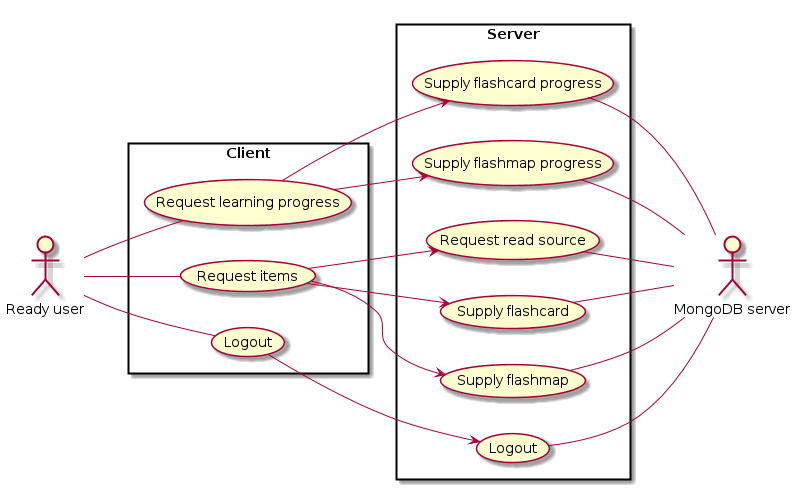
\includegraphics[width=\textwidth]{img/mainusecase.png}
\caption{Use case diagram for main purposes}
\label{fig:mainusecase}
\end{figure}

\paragraph{Learning use cases} The main use cases entail requesting items for review, requesting the learning progress, or logging out. When requesting items for review, the user can receive a due or new flashcard or flashmap, depending whether there are any old items due for review and the experimental group the user is in. Alternatively, the user can also be prompted whether a certain section of the instruction material has been read, since the rehearsal of items cannot be meaningful when the user is not familiar with the content. These prompts take often place at the beginning of a session so that the user does not have to interrupt a session. Furthermore, they prompt two sections ahead of the material currently being learned or reviewed by the user from the flashmap or flashcards in order to guarantee that the user is familiar with the material before learning the items. The user is prompted to read a section at most once per day. After the user has submitted a response, he can undo this response if he is not content with it. For example, the user could after seeing the correct response decide that he thought of a similar enough answer, but after deeper reflection still decide that his answer was not sufficient. In this case, he could use the undo option in order to be presented with the previous response again and select the 'incorrect' option.

\paragraph{Learning progress} When requesting the learning progress, the user is presented of an overview of what has already been learned and what is still left as either unseen items or items due for review. This provides an indication for the user so that he can estimate how much time he still needs to invest into the software, but also could stimulate the user by seeing the number of new or due items lowering and learned items increasing.

Finally, the user can return to the login screen by logging out.

\section{Detailed description of the client server interaction}

Based on the previous description of use cases, there are two sets of complex interaction between the client and server, which are again the interaction for the login and registering process, and the interaction for the learning process. These are described as activity diagrams in figure~\ref{fig:loginactivity} and figure~\ref{fig:learningactivitygen}. These diagrams are elaborated on below together with the specific network messages belonging to the interaction step. Each network message is a simple JSON message consisting of a \emph{keyword} field --- containing the main function which has to be performed by the other party --- and a \emph{data} field containing a dictionary with necessary supplementary data.

\subsection{Login activities}

\begin{figure}[h!]
\centering
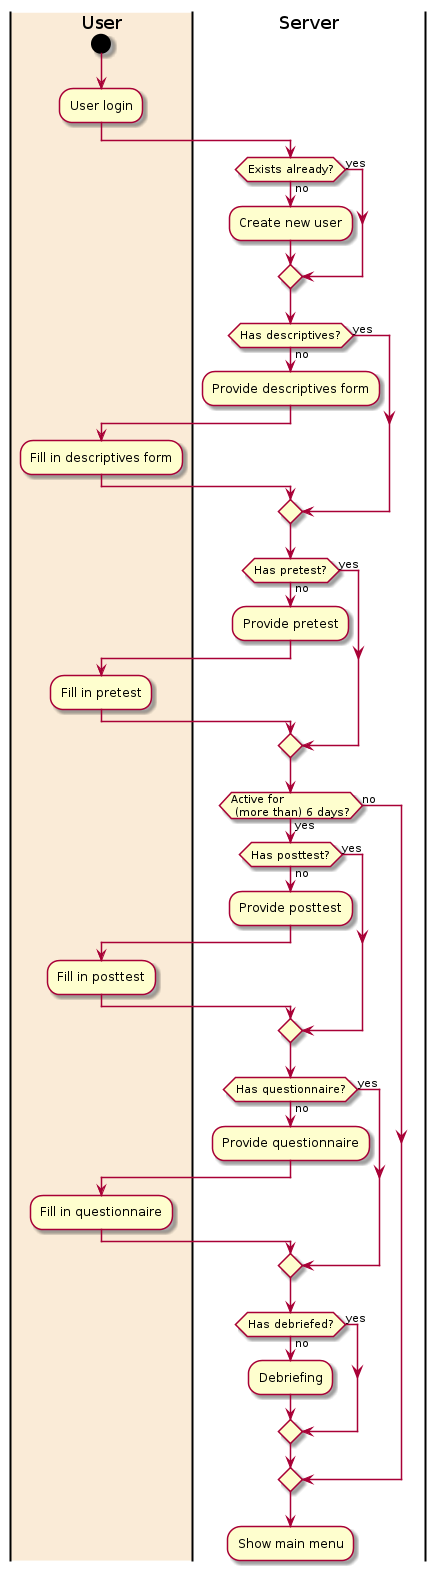
\includegraphics[height=\textheight-10ex]{img/loginactivity.png}
\caption{An activity diagram displaying the server-client interactions when a user logs in}
\label{fig:loginactivity}
\end{figure}

The exact reasoning behind the different activities can be found in the \nameref{sec:procedure} and \nameref{sec:instrumentation} sections of the \nameref{ch:methods} chapter on pages~\pageref{sec:procedure} and \pageref{sec:instrumentation}.

\paragraph{Authenticate} When the user logs in, the client sends a message with keyword "AUTHENTICATE-REQUEST" and data containing a name field with the username. When a user with this username does not exist yet, the server creates a new user with a randomly assigned condition (either flashcard or flashmap, also known as control or experimental). When this user already exists, the server fetches this user from the database.

\paragraph{Descriptives} The server then checks whether the user already has set description fields. If not, the server returns a message with keyword "DESCRIPTIVES-REQUEST", on which the client responds with keyword "DESCRIPTIVES-RESPONSE" with the data fields gender, birthdate, and code.

\paragraph{Pretest} When the previous condition is met, the server will check whether the user has a registered pretest. If this is not the case, it will create a new test by randomly selecting 5 items from the flashcard dataset and 5 items from the itembank, which it will then send to the user with the keyword "TEST-REQUEST". After the user has answered the questions, the client sends the responses to the server with the keyword "TEST-RESPONSE".

\paragraph{After the experiment} If the previous condition is also met, the user will be directed towards the main application with an "AUTHENTICATE-RESPONSE" message from the server, unless he has used the software for at least 15 minutes on 6 days. In that case the checks described below will be performed.

\paragraph{Posttest} In this step the server checks whether the user also has a posttest entry. When this is not the case, it will send a similar test message to the pretest message, with the exception that the flashcards and test items from the pretest are excluded from the random selection in the posttest.

\paragraph{Questionnaire} Sequentially, if the user has no questionnaire entry, the server will construct a new questionnaire by shuffling the Perceived Usefulness item, randomly selecting for each item whether it is positively phrased or negatively, copying this item set but with the opposite phrasing, and finally shuffeling the second set. The same is done for the Perceived Ease of Use items. This questionnaire is then sent to the client with the "QUESTIONNAIRE-REQUEST" keyword. The client sends a filled in version back with the "QUESTIONNAIRE-RESPONSE" keyword to the server with an extra textfield for what was good about the software, what could improved about the software, and an (optional) emailadress of the user for an interview at a later time.

\paragraph{Debriefing} Finally, if the user has not debriefed before, the server sends a message with the keyword "DEBRIEFING-REQUEST" to the client, which will show a debriefing message to the user and returning a message with the keyword "DEBRIEFING-RESPONSE". When all the checks are met, the user will be directed to the main application with the "AUTHENTICATE-RESPONSE" message.

\subsection{Learning activities}

\begin{figure}
\centering
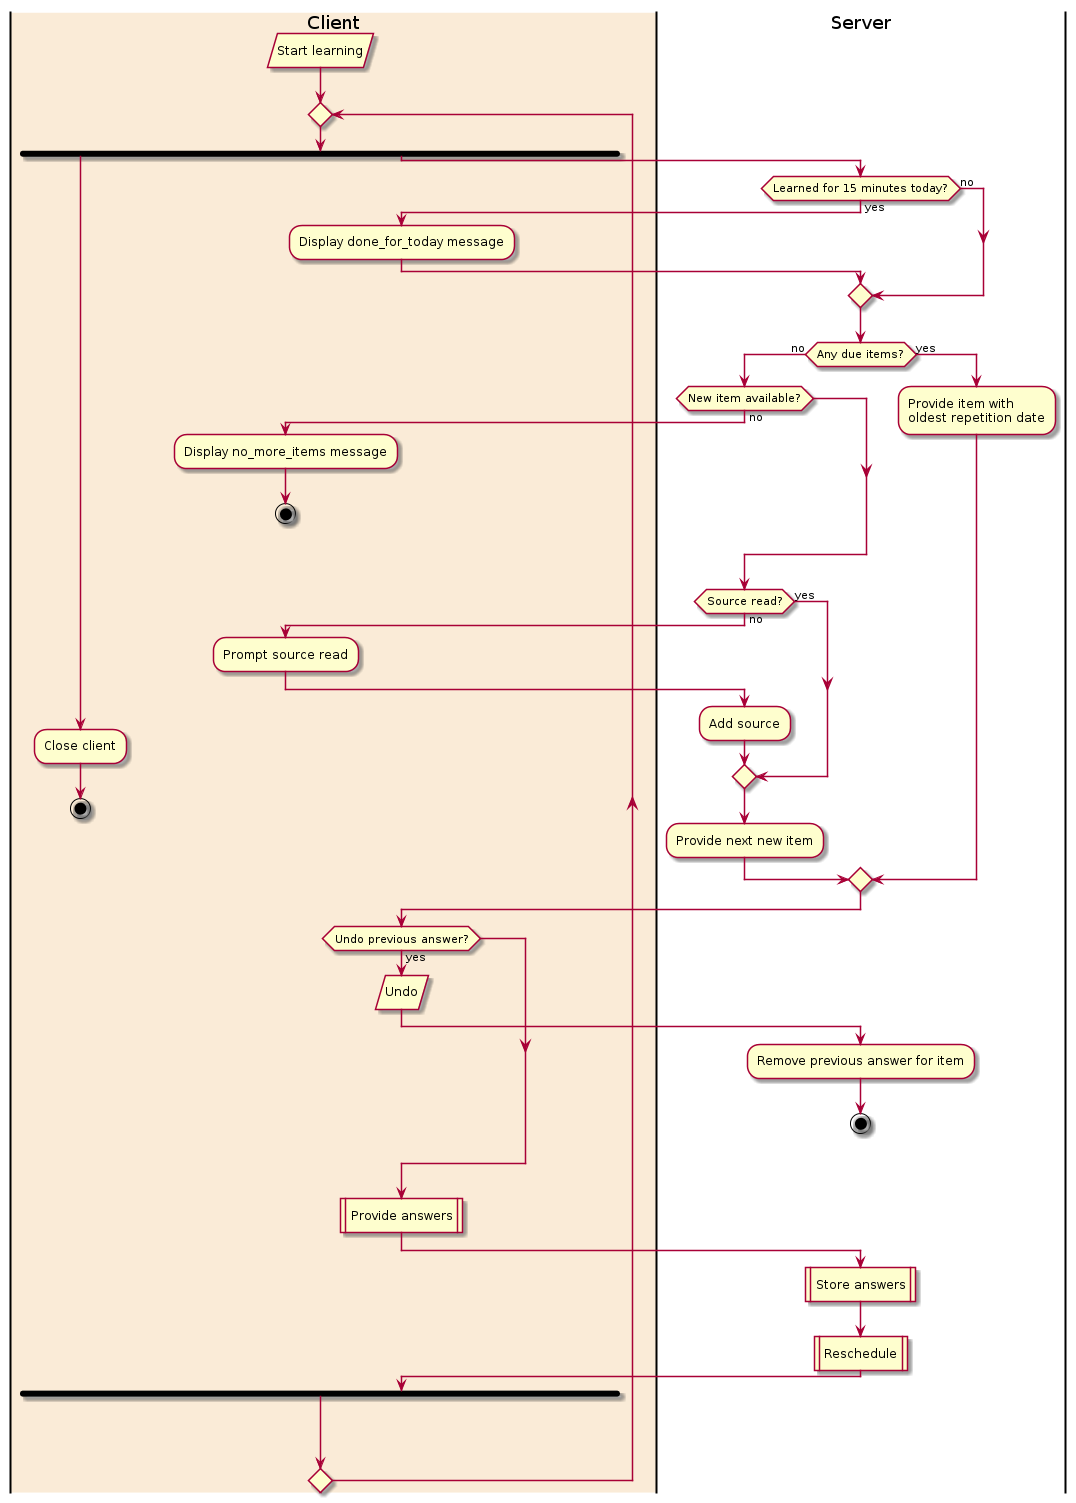
\includegraphics[width=.9\textwidth]{img/learningactivitygen.png}
    \caption{An activity diagram describing the general server-client interactions related to reviewing items. The \protect\emph{Provide answers} activity is described more detailed in figure~\protect\ref{fig:learningclient} on page~\protect\pageref{fig:learningclient}, and the \protect\emph{Store answers} and \protect\emph{Reschedule} activities in figure~\protect\ref{fig:learningserver} on page~\protect\pageref{fig:learningserver}}
\label{fig:learningactivitygen}
\end{figure}

In the main application view, the user can either review items or view his learning progress. If he chooses the latter, a message will be sent to the server with the "LEARNED\_ITEMS-REQUEST" keyword, to which the server will respond with a "LEARNED\_ITEMS-RESPONSE" message containing information on the learning progress (see the \nameref{sec:learningprogress} section on page~\pageref{sec:learningprogress}). If the user wants to review items, the client will send a "LEARN-REQUEST" message to the server and the process described below is performed.

\paragraph{Aimed time reached} First, the server checks whether the user already spent 15 minutes learning today. If this is the case, the client will display a message that the user has spent an sufficient amount of time on learning for today. This will not be directly be displayed as the activity diagram suggests, but rather it will show this message together with the next item.

\paragraph{Selecting an item} After this, the server will check whether there is any item already due for review. If this is the case, the server will sent the item which is due for the longest time to the client with the keyword "LEARN-RESPONSE". If not, the server selects a new item from the database. It is then checked whether the user already read the section in the book related to this item. If not, the server sends a "READ\_SOURCE-REQUEST" to the client, which prompts the user whether he has read the source supplied in the source field of the message. If so, the client sends a "READ\_SOURCE-RESPONSE" message back to the server, which adds the supplied source to the list of read sources for the user. When the user has read the section , the server will sent a "LEARN-RESPONSE" message with a new item from the database. If there is no new item left, the server sends a message to the client with the keyword "NO\_MORE\_INSTANCES".


\paragraph{Validating the item} When the user has reviewed the item, the client sents a "VALIDATE" message to the server with an 'id' field with the item id and a 'correct' field with information whether the user was able to think of the correct response for the item. This response will then be stored in the database by the server, and the item will be rescheduled for when it is due for the next review. After this, the server will repeat the learning cycle as if the client just sent a "LEARN-REQUEST" message.

\paragraph{Undo previous response} When the supplied item is not the first item within the current learning section, the user can choose to undo the response of the previous item. The client will then send back a "UNDO" message to the server, which will then remove the previous response and also go back to the beginning of the learning cycle.
